\section {Systemarchitektur}
\author{Benjamin Besic}

\begin{figure}[htp]
    \centering
    \author{David Ignjatovic}
    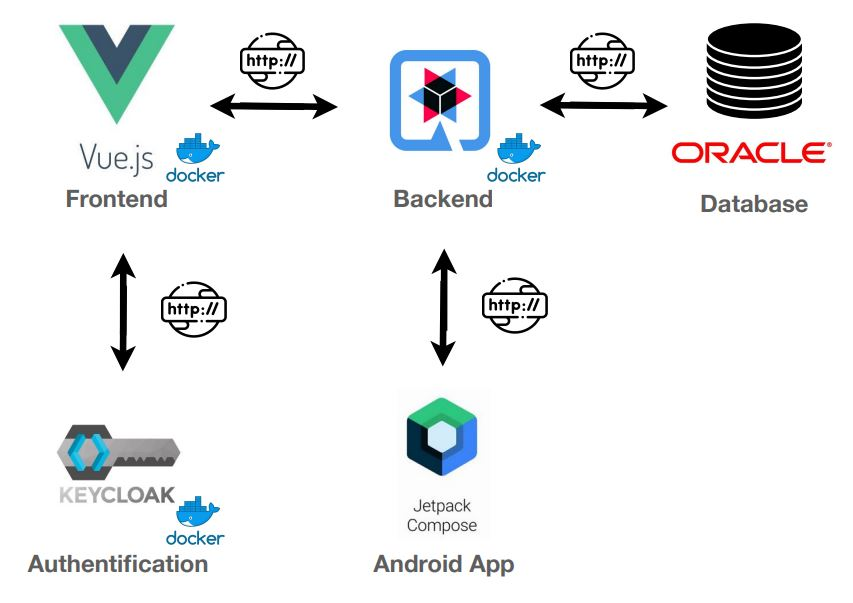
\includegraphics[scale=0.7]{pics/sys-arc-new.JPG}
    \caption{Systemarchitektur des Programms}
    \label{fig:impl:SysArc}
\end{figure}


\section {Webapp}

\subsection{Datenmodell}

\subsection{REST-Schnittstellen}

\subsection{Authentifizierung}

\subsection {Interface}
\subsubsection{Login}
Beim Aufrufen der Webapp wird man zunächst zu der Login-Seite weitergeleitet. Wie diese fungiert, sieht man in der nächsten Abbildung. \\*
Der Login dient in erster Hinsicht dazu, um festzustellen ob der Benutzer ein Mitarbeiter oder Kantinenmitarbeiter ist.
Denn nach dem Login wird man entweder zur Mitarbeiter-Ansicht oder Kantinenmitarbeiter-Ansicht weitergeleitet. \\*
*Abbildung Login*

\subsubsection {Mitarbeiter-Ansicht}

\textbf{Home} \\*
Das Erste, was ein Mitarbeiter zu sehen bekommt, ist die Home Ansicht. In dieser Ansicht ist eine Kalender und die Menüauswahl enthalten. \\*
Der Benutzer kann im Kalender das gewünschte Bestelldatum anklicken, dadurch wird automatisch die Menüauswahl aktualisiert. Man kann sich in die Zukunft, sowohl auch 
in die Vergangenheit klicken, um sich Auskunft über die vergangenen/kommenden Menüs zu beschaffen. Die Ansicht ist nur auf die Bestelltage beschränkt, an denen Menüs angeboten werden.\\*
Nach der erfolgreichen Datumswahl hat man unten drei Menüs zur Auswahl, sowohl wie die dazugehörige Vor- und Nachspeise. Wenn die Bedingungen für eine Bestellung erfüllt sind,
kann man auf einen der drei Bestellknöpfe drücken, um zur Bestellansicht weitergeleitet zu werden. Sind diese Bedingungen nicht erfüllt, sind die Knöpfe ausgeschaltet. \\*
Weiters werden unter den Menüs noch relevante Informationen angezeigt. Durch das Klicken des Fragezeichen-Knopfs wird ein Bild der 14 Allergene geöffnet.

\begin{figure}[htp]
    \centering
    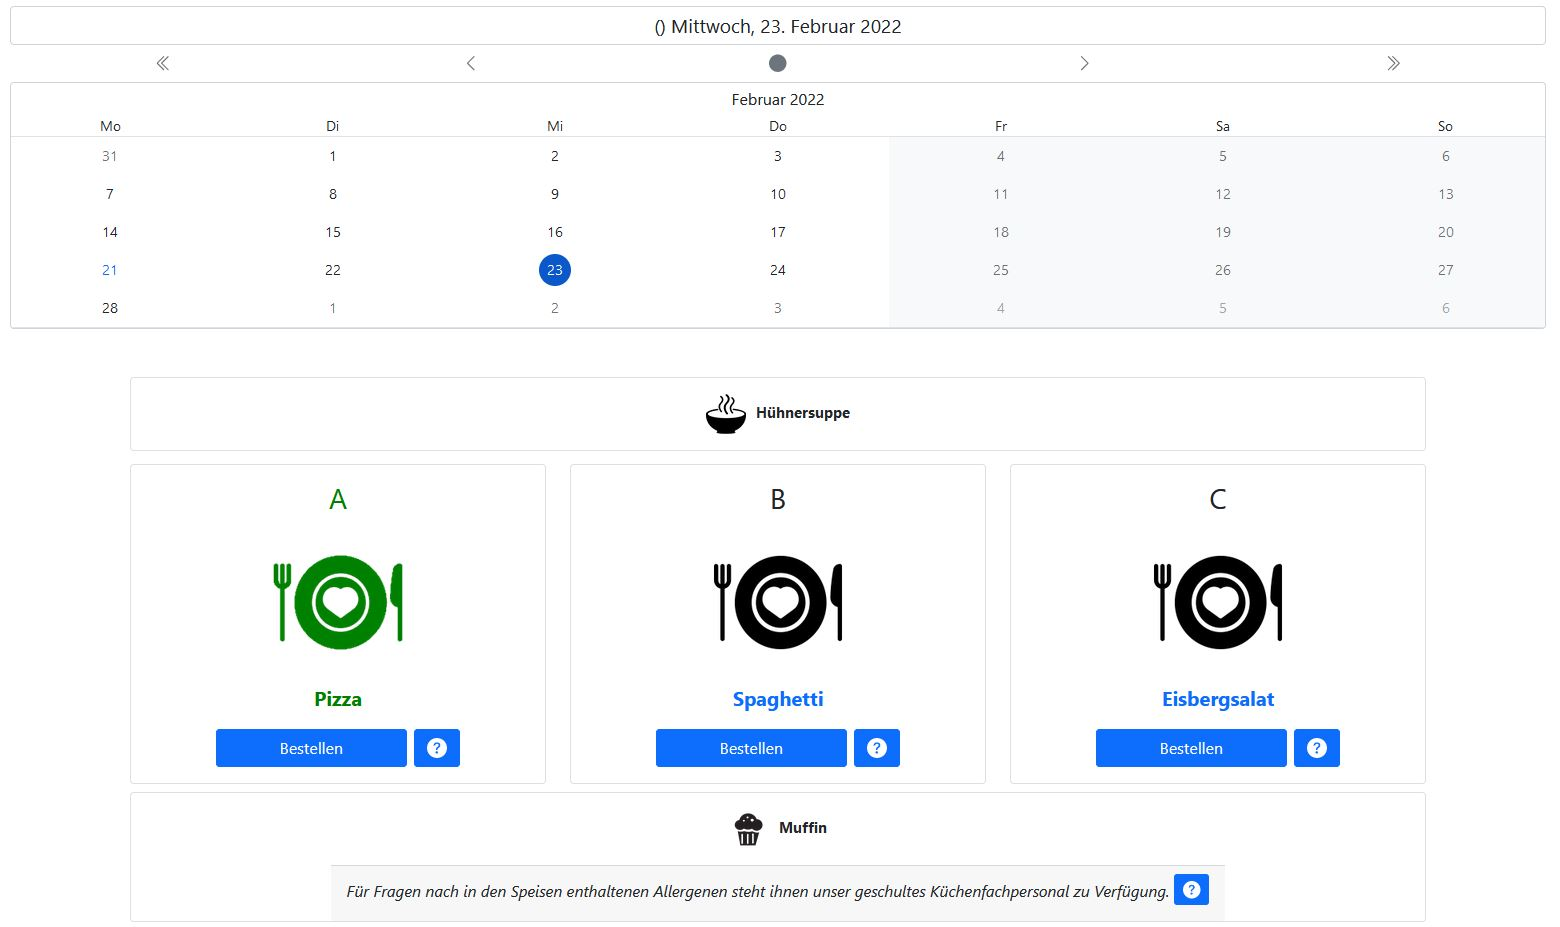
\includegraphics[scale=0.35]{pics/mitarbeiter-home.JPG}
    \caption{Home Ansicht eines Mitarbeiters}
    \label{fig:impl:HomeMitarbeiter}
\end{figure}

\pagebreak

\textbf{Bestellansicht} \\*

In der Bestellansicht werden die nötigen Daten für die Bestellung ausgefüllt. Die ersten drei Felder sind automatisch ausgefüllt, aufgrund der vorherigen Auswahl. \\*
Die Tabelle auf der rechten Seite enthält alle Bestellzeiträume, die es gibt. Man kann nur eine gleichzeitig auswählen. Außerdem stehen die freien Plätze dabei, die aus der Datenbank geladen werden.\\*
Die Anzahl der Menüs kann durchs Klicken des Plus- und Minusknopfs angepasst werden.  \\*
Darunter steht voreingestellt der Benutzer, doch dies kann verändert werden, um das Menü für einen anderen Mitarbeiter bestellen zu können. \\*
Abschließend kann man noch einen Kommentar an die Kantine mitgeben, falls es etwaige Extrawünsche geben sollte. \\*
Die Bestellung kann durch den Abschließen-Knopf durchgeführt werden und Abbrechen kann man jederzeit mit dem Abbrechen-Knopf.
Die Bestellung ist erst ausführbar, sobald alle Felder außer des Kommentars ausgefüllt wurden.
\begin{figure}[htp]
    \centering
    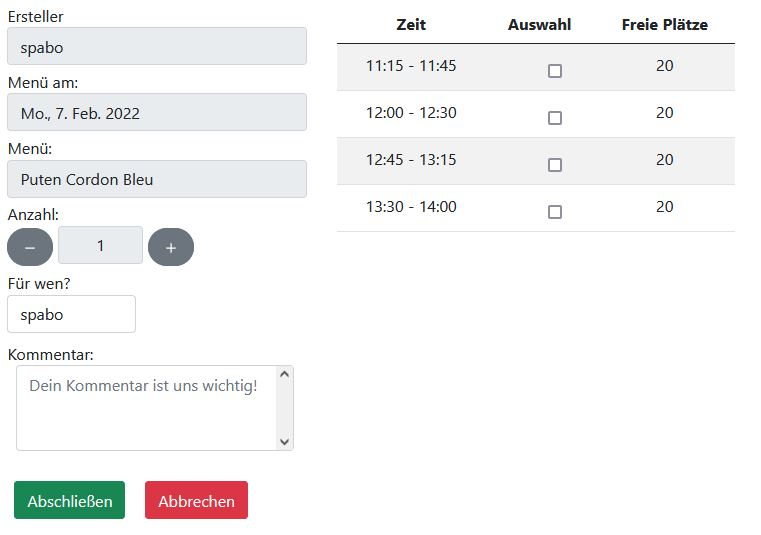
\includegraphics[scale=0.6]{pics/mitarbeiter-bestellen.JPG}
    \caption{Bestellansicht}
    \label{fig:impl:BestellenMitarbeiter}
\end{figure}
\pagebreak

\textbf{Bestellübersicht} \\*

\begin{figure}[htp]
    \centering
    \includegraphics[scale=0.4]{pics/mitarbeiter-bestellen-übersicht.JPG}
    \caption{Bestellungsübersicht}
    \label{fig:impl:BestellenMitarbeiterUebersicht}
\end{figure}

\section{Android App}